\begin{frame}
  \frametitle{Substepping}
  \cite{slimani2025}:
  \begin{itemize}
    \item Examines SOA of substepping methods for LPBF;
      identifies common structures and shortcomings.
    \item New Robin-Robin substepper for LPBF is compared against
      Dirichlet substepper of \cite{hodge2021}.
    \item Realistic speedup estimates provided.
    \item Alternate predictor schemes are proposed and tested.
    \item Robin-Robin version of AS method is proposed.
    \item AS is nested within the fast partition of said substeppers.
  \end{itemize}
\end{frame}

\begin{frame}
  \frametitle{Substepping + advected subdomain}
  \begin{figure}
    \centering
    \seudoembeddedvod{width=1.0\textwidth}{videos/basic-demo-css.mp4}{thumbnail-basic-css.png}
    \caption{Basic demo of combined substepping + advected subdomain method.}
  \end{figure}
\end{frame}

\begin{frame}
  \frametitle{Substepping}
  \framesubtitle{Example time-step}
  \begin{figure}
    \begin{subfigure}[t]{0.46\textwidth}
      \centering
      \includegraphics[width=\textwidth]{{ss_robin/prev_sol.png}}
      \caption{$T^{n}$}
      \label{fig:robin_prev}
    \end{subfigure}%
    \hfill%
    \begin{subfigure}[t]{0.46\textwidth}
      \centering
      \includegraphics[width=\textwidth]{{ss_robin/predictor.png}}
      \caption{$\tilde{T}^{n+1}$ after predictor step}
      \label{fig:robin_predictor}
    \end{subfigure}
    \caption{Previous solution and predictor step.}
  \end{figure}
\end{frame}

\begin{frame}
  \frametitle{Substepping}
  \framesubtitle{Example time-step}
  \begin{figure}
  \begin{subfigure}[t]{0.46\textwidth}
    \centering
    \includegraphics[width=\textwidth]{{ss_robin/micro_step.png}}
    \caption{Intermediate \textbf{Robin} substep.}
    \label{fig:robin_substep}
  \end{subfigure}%
  \hfill%
  \begin{subfigure}[t]{0.46\textwidth}
    \centering
    \begin{tikzpicture}
      \node[anchor=south west, inner sep=0] (A) {\includegraphics[width=\textwidth]{{ss_robin/macro_step.png}}};
    \begin{scope}[x={(A.south east)},y={(A.north west)}]
      % Rectangle highlight (coordinates between 0 and 1)
      %\draw[teal!20, step=0.05] (0,0) grid (1,1);%grid, comment out for draft
      \draw[red, thick, dash pattern=on 1pt off 1pt] (0.286, 0.5475) circle (0.02);
      \draw[red, thick, dash pattern=on 1pt off 1pt] (0.286, 0.6385) circle (0.02);
    \end{scope}
    \end{tikzpicture}
    \caption{\textbf{Robin} corrector step.}
    \label{fig:robin_corrector}
  \end{subfigure}
  \caption{Robin-Robin substepper.}
  \end{figure}
\end{frame}

\begin{frame}
  \frametitle{Substepping}
  \framesubtitle{Example time-step}
  \begin{figure}
    \begin{subfigure}[t]{0.46\textwidth}
      \centering
      \begin{tikzpicture}
        \node[anchor=south west, inner sep=0] (A) {\includegraphics[width=\textwidth]{{hodge/micro_step.png}}};
      \begin{scope}[x={(A.south east)},y={(A.north west)}]
        % Rectangle highlight (coordinates between 0 and 1)
        %\draw[teal!20, step=0.01] (0,0) grid (1,1);%grid, comment out for draft
        \draw[red, thick, dash pattern=on 1pt off 1pt, rounded corners] (0.0625, 0.450) rectangle (0.2, 0.5);
        \draw[red, thick, dash pattern=on 1pt off 1pt, rounded corners] (0.2500, 0.5505) rectangle (0.3100, 0.7100);
      \end{scope}
      \end{tikzpicture}
      \caption{Intermediate \textbf{Dirichlet} substep. The Dirichlet
      condition does not let the solution deviate from the predictor.}
      \label{fig:hodge_substep}
    \end{subfigure}%
    \hfill%
    \begin{subfigure}[t]{0.46\textwidth}
      \centering
      \begin{tikzpicture}
        \node[anchor=south west, inner sep=0] (A) {\includegraphics[width=\textwidth]{{hodge/macro_step.png}}};
      \begin{scope}[x={(A.south east)},y={(A.north west)}]
        % Rectangle highlight (coordinates between 0 and 1)
        %\draw[teal!20, step=0.01] (0,0) grid (1,1);%grid, comment out for draft
        \draw[red, thick, dash pattern=on 1pt off 1pt, rounded corners] (0.065, 0.4550) rectangle (0.1905, 0.4905);
        \draw[red, thick, dash pattern=on 1pt off 1pt, rounded corners] (0.2600, 0.5605) rectangle (0.3000, 0.7000);
      \end{scope}
      \end{tikzpicture}
  \caption{\textbf{Dirichlet} corrector step.}
  \label{fig:hodge_corrector}
\end{subfigure}
    \caption{Dirichlet substepper of \cite{hodge2021}.}
  \end{figure}
\end{frame}

\begin{frame}
  \frametitle{Substepping}
  \framesubtitle{No heat source predictor}

  \begin{figure}
    \begin{subfigure}[t]{0.33\textwidth}
      \centering
      \includegraphics[width=\textwidth]{hodge/to_predictor.png}
      \caption{Predictor step without heat input}
      \label{fig:to_hodge_predictor}
    \end{subfigure}%
    \hfill
    \begin{subfigure}[t]{0.33\textwidth}
      \centering
      \includegraphics[width=\textwidth]{hodge/to_micro_step.png}
      \caption{Micro-step.}
      \label{fig:to_hodge_micro}
    \end{subfigure}%
    \hfill
    \begin{subfigure}[t]{0.33\textwidth}
      \centering
      \includegraphics[width=\textwidth]{hodge/to_macro_step.png}
      \caption{Corrector step.}
      \label{fig:to_hodge_macro}
    \end{subfigure}
    \caption{Example of Dirichlet substepper step using a predictor step without including the source term.}
    \label{fig:to_hodge}
  \end{figure}
\end{frame}

\begin{frame}
  \frametitle{Substepping}
  \framesubtitle{2D square track}

    \begin{adjustwidth}{-10mm}{-10mm}
    \begin{figure}
    \centering
    \begin{tabular}{cccc}
      \begin{subfigure}[t]{0.28\textwidth}
        \centering
        \begin{tikzpicture}
          \node[anchor=south west, inner sep=0] (image) at (0, 0) {
            \includegraphics[width=\textwidth, clip=true, trim={0cm 0cm 12cm 0cm}]{{2d_square_track/sols/linear_ref_pred0_16els_tf0_5_ts8_0_time0_0032.png}}
          };
        \end{tikzpicture}
        \caption{Solution -- No substepping.}
        \label{fig:sol_ref_t4}
      \end{subfigure}
      &
      \begin{subfigure}[t]{0.28\textwidth}
        \centering
        \begin{tikzpicture}
          \node[anchor=south west, inner sep=0] (image) at (0, 0) {
            \includegraphics[width=\textwidth, clip=true, trim={0cm 0cm 12cm 0cm}]{{2d_square_track/sols/robin_linear_ss_rr_pred0_16els_tf0_5_ts8_0_time0_0032.png}}
          };
        \node[text opacity=1] at ($(image.west)!0.35!(image.east) + (0.0, 0.0)$) {\labelbox{$\Omega_f$}};
        \end{tikzpicture}
        \caption{Solution -- Robin.}
        \label{fig:sol_robin_t4}
      \end{subfigure}
      &
      \begin{subfigure}[t]{0.28\textwidth}
        \centering
        \begin{tikzpicture}
          \node[anchor=south west, inner sep=0] (image) at (0, 0) {
            \includegraphics[width=\textwidth, clip=true, trim={0cm 0cm 12cm 0cm}]{{2d_square_track/sols/chimera_ss_RR_linear_css_pred0_16els_tf0_5_ts8_0_time0_0032.png}}
          };
          \node[text opacity=1] at ($(image.west)!0.35!(image.east) + (0.0, 0.0)$) {\labelbox{$\Omega_f$}};
          \node[text opacity=1, anchor=south, inner sep=1pt] at ($(image.south west)!0.36!(image.south east) + (0.0, 0.0)$) {\labelbox{$\Omega_m$}};
        \end{tikzpicture}
        \caption{Solution -- Robin with AS.}
        \label{fig:sol_chimera_robin_t4}
      \end{subfigure}
      &
      \begin{subfigure}[t]{0.1\textwidth}
        \raisebox{0.1\height}{
          \vcolorbar{rainbow_blended_white}{0.2cm}{25}{2000}{$u_h$}{}
        }
      \end{subfigure}
      \\[5mm]
      \begin{subfigure}[t]{0.28\textwidth}
        \centering
        \includegraphics[width=\textwidth, clip=true, trim={0cm 0cm 12cm 0cm}]{{2d_square_track/errs/linear_ref_pred0_16els_tf0_5_ts8_0_time0_0032.png}}
        \caption{Squared error -- No substepping.}
        \label{fig:err_ref_t4}
      \end{subfigure}
      &
      \begin{subfigure}[t]{0.28\textwidth}
        \centering
        \includegraphics[width=\textwidth, clip=true, trim={0cm 0cm 12cm 0cm}]{{2d_square_track/errs/robin_linear_ss_rr_pred0_16els_tf0_5_ts8_0_time0_0032.png}}
        \caption{Squared error -- Robin.}
        \label{fig:err_robin_t4}
      \end{subfigure}
      &
      \begin{subfigure}[t]{0.28\textwidth}
        \centering
        \includegraphics[width=\textwidth, clip=true, trim={0cm 0cm 12cm 0cm}]{{2d_square_track/errs/chimera_ss_RR_linear_css_pred0_16els_tf0_5_ts8_0_time0_0032.png}}
        \caption{Squared error -- Robin with AS.}
        \label{fig:err_chimera_robin_t4}
      \end{subfigure}
      &
      \begin{subfigure}[t]{0.1\textwidth}
        \raisebox{0.1\height}{
        \vcolorbar{fast}{0.2cm}{0}{10000}{$(u_h - u_{ex})^2$}{}
        }
      \end{subfigure}
    \end{tabular}
    % \caption{Solutions (top row) and pointwise squared errors (bottom row) in the linear case for the Robin substepper
    %   with and without an AS, with $\Delta t_s = 8 T_{hs}$ and $\Delta t_f = 0.5 T_{hs}$.
    %   The unsubstepped solution with $\Delta t = 0.5 T_{hs}$ is shown for reference.
    %   The substeppers introduce some error throughout the domain.
    %   The advected subdomain reduces the error in the HAZ but increases the error near the track turns.
    % }
    \label{fig:err_linear_vsadvected}
  \end{figure}
  \end{adjustwidth}
\end{frame}

\begin{frame}
  \frametitle{Substepping}
  \framesubtitle{2D square track}
  \begin{figure}[ht]
  \centering
  \pgfplotslegendfromname{legendmidline}\\[1em]
  \begin{subfigure}[t]{0.5\linewidth}
    \centering
    \begin{tikzpicture}[
        trim axis left,
        trim axis right,
        baseline,
    ]
    \begin{axis}[
      width=1.0\linewidth,
      oscillationstyle,
      legend to name=legendmidline,
      legend cell align=left,
      legend style={font=\footnotesize,
        /tikz/every even column/.append style={column sep=0.5cm},
        legend columns=3,
        transpose legend,
      },
      legend image post style={xscale=0.8, yscale=0.8},
    ]
      \addlegendentry{Dirichlet, $\Delta t_s = 4 T_{hs}$}
      \addplot+
      [mark=none, opacity=0.8]
      table [col sep=comma, x=x, y=uh] {./plots/2dsquare_midline/midline_CSVs/smslinear-Ths=4-midline.csv};

      \addlegendentry{Dirichlet, $\Delta t_s = 8 T_{hs}$}
      \addplot+
      [mark=none, opacity=0.8]
      table [col sep=comma, x=x, y=uh] {./plots/2dsquare_midline/midline_CSVs/smslinear-Ths=8-midline.csv};

      \addlegendentry{Dirichlet, $\Delta t_s = 16 T_{hs}$}
      \addplot+
      [mark=none, opacity=0.8]
      table [col sep=comma, x=x, y=uh] {./plots/2dsquare_midline/midline_CSVs/smslinear-Ths=16-midline.csv};

      \addlegendentry{Robin, $\Delta t_s = 4 T_{hs}$}
      \addplot+
      [mark=none, opacity=0.8, unbounded coords=jump]
      table [col sep=comma, x=x, y=uh] {{plots/2dsquare_midline/midline_CSVs/ssrobinlinear-Ths=4-midline.csv}};

      \addlegendentry{Robin, $\Delta t_s = 8 T_{hs}$}
      \addplot+
      [mark=none, opacity=0.8, unbounded coords=jump]
      table [col sep=comma, x=x, y=uh] {{plots/2dsquare_midline/midline_CSVs/ssrobinlinear-Ths=8-midline.csv}};

      \addlegendentry{Robin, $\Delta t_s = 16 T_{hs}$}
      \addplot+
      [mark=none, opacity=0.8, unbounded coords=jump]
      table [col sep=comma, x=x, y=uh] {{plots/2dsquare_midline/midline_CSVs/ssrobinlinear-Ths=16-midline.csv}};
    \end{axis}
    \end{tikzpicture}
    \caption{Linear case.}
    \label{fig:midline_linear}
  \end{subfigure}%
  \begin{subfigure}[t]{0.5\linewidth}
    \centering
    \begin{tikzpicture}[
        trim axis left,
        trim axis right,
        baseline,
    ]
    \begin{axis}[
      width=1.0\linewidth,
      oscillationstyle,
      yticklabel={$$},
      ylabel={},
      y unit={},
    ]
      \addplot+
      [mark=none, opacity=0.8]
      table [col sep=comma, x=x, y=uh] {./plots/2dsquare_midline/midline_CSVs/smsnnlinear-Ths=4-midline.csv};
      \addplot+
      [mark=none, opacity=0.8]
      table [col sep=comma, x=x, y=uh] {./plots/2dsquare_midline/midline_CSVs/smsnnlinear-Ths=8-midline.csv};
      \addplot+
      [mark=none, opacity=0.8]
      table [col sep=comma, x=x, y=uh] {./plots/2dsquare_midline/midline_CSVs/smsnnlinear-Ths=16-midline.csv};

      \addplot+
      [mark=none, opacity=0.8, unbounded coords=jump]
      table [col sep=comma, x=x, y=uh] {{plots/2dsquare_midline/midline_CSVs/ssrobinnnlinear-Ths=4-midline.csv}};

      \addplot+
      [mark=none, opacity=0.8, unbounded coords=jump]
      table [col sep=comma, x=x, y=uh] {{plots/2dsquare_midline/midline_CSVs/ssrobinnnlinear-Ths=8-midline.csv}};

      \addplot+
      [mark=none, opacity=0.8, unbounded coords=jump]
      table [col sep=comma, x=x, y=uh] {{plots/2dsquare_midline/midline_CSVs/ssrobinnnlinear-Ths=16-midline.csv}};
    \end{axis}
    \end{tikzpicture}
    \caption{Non-linear case.}
    \label{fig:midline_nnlinear}
  \end{subfigure}

  \caption{Solution profiles along first heating track
  for increasing $\Delta t_s$ and constant $\Delta t_f = \tfrac{1}{8} T_{hs}$,
  for both substeppers without AS.}
  \label{fig:1sttrackmidline}
\end{figure}

\end{frame}

\begin{frame}
  \frametitle{Substepping}
  \framesubtitle{2D square track}
  \begin{adjustwidth}{-7mm}{-5mm}
    \begin{figure}
  \centering
  \begin{tikzpicture}[
      baseline,
      spy using outlines= {circle, connect spies},
    ]
    \begin{groupplot}[
      group style={
        group size=3 by 1,
        horizontal sep=0.4cm,
      },
    ]
    \nextgroupplot[
      truncatedddstyle,
      legend style={legend columns=2, at={(0.5,0.02)}, anchor=south},
      width=0.31\textwidth,
      legend cell align=left,
      title={Dirichlet-Neumann},
      ]

      \gammafs{}

      \addlegendentry{Iter. 1}
      \addplot+[mark=none, thin, unbounded coords=jump, opacity=0.8]
      table [col sep=comma, x=x, y=uh] {./plots/truncated_iters/CSVs/ssdnaitken_relax-midline-t1.csv};
      \addlegendentry{Iter. 2}
      \addplot+[mark=none, thin, unbounded coords=jump, opacity=0.8]
      table [col sep=comma, x=x, y=uh] {./plots/truncated_iters/CSVs/ssdnaitken_relax-midline-t2.csv};
      \addlegendentry{Iter. 4}
      \addplot+[mark=none, thin, unbounded coords=jump, opacity=0.8]
      table [col sep=comma, x=x, y=uh] {./plots/truncated_iters/CSVs/ssdnaitken_relax-midline-t4.csv};
      \addlegendentry{Iter. 8}
      \addplot+[mark=none, thin, unbounded coords=jump, opacity=0.8]
      table [col sep=comma, x=x, y=uh] {./plots/truncated_iters/CSVs/ssdnaitken_relax-midline-t8.csv};
    \nextgroupplot[
      truncatedddstyle,
      ylabel={},
      y unit={},
      yticklabel={$$},
      width=0.31\textwidth,
      legend pos=south east,
      legend cell align=left,
      title={Robin},
      ]

      \gammafs{}

      \addlegendentry{Iter. 1}
      \addplot+[mark=none, thin, unbounded coords=jump, opacity=0.8]
      table [col sep=comma, x=x, y=uh] {./plots/truncated_iters/CSVs/ssrobin-midline-t1.csv};
      \addlegendentry{Iter. 2}
      \addplot+[mark=none, thin, unbounded coords=jump, opacity=0.8]
      table [col sep=comma, x=x, y=uh] {./plots/truncated_iters/CSVs/ssrobin-midline-t2.csv};

      \coordinate (spypointrobin) at (axis cs:-0.15,  1418.0);
      \coordinate (magnifyglassrobin) at (axis cs:-0.5,  1900.0);
    \nextgroupplot[
      truncatedddstyle,
      legend style={legend columns=2},
      ylabel={},
      y unit={},
      yticklabel={$$},
      width=0.31\textwidth,
      legend pos=south east,
      legend cell align=left,
      title={Dirichlet},
      ]

      \gammafs{}

      \addlegendentry{Iter. 1}
      \addplot+[mark=none, thin, unbounded coords=jump, opacity=0.8]
      table [col sep=comma, x=x, y=uh] {./plots/truncated_iters/CSVs/sms-midline-t1.csv};
      \addlegendentry{Iter. 2}
      \addplot+[mark=none, thin, unbounded coords=jump, opacity=0.8]
      table [col sep=comma, x=x, y=uh] {./plots/truncated_iters/CSVs/sms-midline-t2.csv};
      \addlegendentry{Iter. 4}
      \addplot+[mark=none, thin, unbounded coords=jump, opacity=0.8]
      table [col sep=comma, x=x, y=uh] {./plots/truncated_iters/CSVs/sms-midline-t4.csv};

      \coordinate (spypointsms) at (axis cs:-0.15,  1430.0);
      \coordinate (magnifyglasssms) at (axis cs:-0.5,  1900.0);
  \end{groupplot}

  \spy [black, width=1.5cm, height=1.5cm, magnification=10] on (spypointrobin) in node[fill=white] at (magnifyglassrobin);
  \spy [black, width=1.5cm, height=1.5cm, magnification=10] on (spypointsms) in node[fill=white] at (magnifyglasssms);


\end{tikzpicture}
\caption{Solution profiles along the heating track after multiple staggered
iterations for a linear problem with $\Delta t_s = 8 T_{hs}$ and $\Delta t_f =
0.125 T_{hs}$. Substeppers from left to right: Dirichlet–Neumann with Aitken
relaxation, Robin, and Dirichlet.}
\label{fig:truncated_iters}
\end{figure}

  \end{adjustwidth}
\end{frame}

\begin{frame}
  \frametitle{Substepping}
  \framesubtitle{Experimental validation}
  Validation against experimental melt pool shape data of \cite{lane2020} (AMB2018-02),
  as done in \cite{kopp2022}.\\
  \begin{adjustwidth}{-5mm}{-5mm}
    \begin{figure}
  \begin{subfigure}[b]{0.44\linewidth}
  \centering
  \hcolorbar{rainbow}{0.4cm}{25}{2700}{$T$}{0.485985}\\
  \begin{tikzpicture}
    \node[anchor=south west, inner sep=0] (image) at (0, 0) {
      \includegraphics[width=\linewidth]{ambench_perspective_chimera_stagg.png}
    };
    \node[fill=white, fill opacity=0.7, text opacity=1, inner sep=1pt, rounded corners=2pt] at ($(image.west)!0.5!(image.east) + (2.4, -0.5)$) {$\Omega_m$};
    \node[fill=white, fill opacity=0.7, text opacity=1, inner sep=1pt, rounded corners=2pt] at ($(image.west)!0.9!(image.east) + (0.0, -1.05)$) {$\Omega_f$};
    \node[fill=white, fill opacity=0.7, text opacity=1, inner sep=1pt, rounded corners=2pt] at ($(image.south)!0.9!(image.north) + (2.0, 0.0)$) {$\Omega_s$};
  \end{tikzpicture}
  \caption{Intermediate substep of Robin substepper with an AS.}
  \label{fig:perspective_chimera}
\end{subfigure}%
\quad
\begin{subfigure}[b]{0.52\linewidth}
  \centering
\begin{tikzpicture}[
    spy using outlines= {rectangle, connect spies}
  ]
  \begin{groupplot}[
    group style={
      group size=1 by 2,
      vertical sep=0.6cm, % adjust as needed
    },
    trim axis left,
    trim axis right,
    width=8cm, % set width for both plots
    height=5cm,
    meltpoolstyle,
  ]
    \nextgroupplot[
        xlabel style={at={(axis description cs:1.0, -0.1)},anchor=west},
        x unit=\si{\micro\meter},
        ymin=0.0,
        ymax=+100.0,
        ylabel style={at={(axis description cs:1.05,0.3)},anchor=west},
        legend style={
          at={(0.5, +1.2)},
          anchor=south,
          legend columns=-1,
          cells={align=left},
          font=\footnotesize,
        },
        legend image post style={xscale=0.8},
        title={Top view},
        title style={at={(0.5,0.5)}, anchor=south},
    ]
    \addlegendentry{\citeauthor{kopp2022}}
    \addplot+[mark=none, opacity=0.6, thick]
      table [col sep=comma, x expr=\thisrow{x}*1e6, y expr=\thisrow{y}*1e6] {./plots/meltpool_contours/CSVs/kopp_ulp200_bird_view_sorted.csv} -- cycle;
    \addlegendentry{w/o AS}
    \addplot+[mark=none, opacity=0.6, thick]
      table [col sep=comma, x expr=\thisrow{x}*1e6, y expr=\thisrow{y}*1e6] {./plots/meltpool_contours/CSVs/hodge_8els_s025_bird_view_sorted.csv} -- cycle;
    \addlegendentry{w/ AS}
    \addplot+[mark=none, opacity=0.6, thick]
      table [col sep=comma, x expr=\thisrow{x}*1e3 - 1e3, y expr=\thisrow{y}*1e3] {./plots/meltpool_contours/CSVs/chimera_robin_8els_s025_bird_view_sorted.csv};
    \coordinate (spypoint_bird) at (axis cs:27.5, 0);
    \coordinate (magnifyglass_bird) at (axis cs:30,50);

    \nextgroupplot[
      xticklabels={},
      xlabel style={at={(axis description cs:0.5,1.05)},anchor=south},
      ymin=-50.0,
      ymax=+0.0,
      title={Side view},
      title style={at={(0.5,-0.2)}, anchor=north},
    ]
    \addplot+[mark=none, opacity=0.6, thick]
      table [col sep=comma, x expr=\thisrow{x}*1e4, y expr=\thisrow{y}*1e4] {./plots/meltpool_contours/CSVs/kopp_ulp200_side_view_sorted.csv};
    \addplot+[mark=none, opacity=0.6, thick]
      table [col sep=comma, x expr=\thisrow{x}*1e3 - 1e3, y expr=\thisrow{y}*1e3] {./plots/meltpool_contours/CSVs/robin_8els_s025_side_view_sorted.csv};
    \addplot+[mark=none, opacity=0.6, thick]
      table [col sep=comma, x expr=\thisrow{x}*1e3 - 1e3, y expr=\thisrow{y}*1e3] {./plots/meltpool_contours/CSVs/chimera_robin_8els_s025_side_view_sorted.csv};
    \coordinate (spypoint_side) at (axis cs:-310.0, 0);
    \coordinate (magnifyglass_side) at (axis cs:-304,-25);
  \end{groupplot}
  \spy [black, width=0.7cm, height=0.8cm, anchor=south west, magnification=3]
    on (spypoint_bird) in node[fill=white] at (magnifyglass_bird);
  \spy [black, width=0.9cm, height=0.6cm, anchor=north east, magnification=2.5]
    on (spypoint_side) in node[fill=white] at (magnifyglass_side);
\end{tikzpicture}
  \caption{Top and side views of simulated melt pool contours, with and without AS, compared against results from \cite{kopp2022}.}
  \label{fig:side_kopp_contours}
\end{subfigure}
\end{figure}


  \end{adjustwidth}
\end{frame}

\begin{frame}
  \frametitle{Substepping}
  \framesubtitle{3D LPBF cube}
  \begin{figure}
    \centering
    \begin{subfigure}[b]{0.33\textwidth}
      \centering
      \includegraphics[width=\textwidth]{{stacked_cubes/mesh.png}}
      \caption{Mesh and material composition at start of print.}
      \label{fig:3d_lpbf_mesh}
    \end{subfigure}%
    \hfill
    \begin{subfigure}[b]{0.33\textwidth}
      \centering
      \includegraphics[width=\textwidth]{{stacked_cubes/scan_path.png}}
      \caption{Printing path.}
      \label{fig:3d_lpbf_path}
    \end{subfigure}%
    \hfill
    \begin{subfigure}[b]{0.33\textwidth}
      \centering
      \includegraphics[width=\textwidth]{{stacked_cubes/bulk_mesh.png}}
      \caption{Bulk material at final time.}
      \label{fig:3d_lpbf_bulk_mesh}
    \end{subfigure}
    \caption{\centering \SI{1}{\milli\meter} cube. Powder elements
      corresponding to each layer are activated during recoating time-steps.
    \qquad \legendpowderbulk{}}
  \end{figure}
\end{frame}

\begin{frame}
  \frametitle{Substepping}
  \framesubtitle{3D LPBF cube}

  \vspace{-7mm}
  \definecolor{OIblue}{HTML}{0072B2}
\definecolor{OIverm}{HTML}{E69F00}
\definecolor{OIred}{HTML}{D55E00}
\definecolor{OIgreen}{HTML}{009E73}


\pgfplotsset{
  refstyle/.style={
    very thick, color=OIblue, solid, mark=none,
  },
  staggeredstyle/.style={
    thick, color=OIverm, densely dashed, mark=none,
  },
  dirichletstyle/.style={
    thick, color=OIred, dash pattern=on 7pt off 3pt,
    mark=none,
  },
  chimerastyle/.style={
    thick, color=OIgreen!85!black, densely dotted,
    mark=none,
  },
  layerzerostyle/.style={
    enlarge x limits=false,
    axis x discontinuity=crunch,
    axis x line*=bottom,
    axis y line*=left,
    xtick=\empty,
    clip=false,
    yticklabel style={font=\tiny, /pgf/number format/fixed},
    xticklabel style={font=\tiny},
    grid=major,
  },
  layerstyle/.style={
    layerzerostyle,
    axis y line=none,
    yticklabels=\empty,
    xticklabel style={font=\tiny},
  },
}

\newcommand{\addlayer}[6]{
  \ifnum#1=0
    \nextgroupplot[
      layerzerostyle,
      ylabel={\tiny #3},
      y unit={\tiny #4},
      ymin=#5, ymax=#6,
    ]
  \else
    \nextgroupplot[
      layerstyle,
      ymin=#5, ymax=#6,
    ]
  \fi
  \addplot[refstyle] table [x=time, y=#2, col sep=comma] {{plots/stacked_cubes_probe/ref_layers/layer_#1.csv}};
  \addplot[staggeredstyle] table [x=time, y=#2, col sep=comma] {{plots/stacked_cubes_probe/robin_layers/layer_#1.csv}};
  \addplot[dirichletstyle] table [x=time, y=#2, col sep=comma] {{plots/stacked_cubes_probe/hodge_layers/layer_#1.csv}};
  \addplot[chimerastyle] table [x=time, y=#2, col sep=comma] {{plots/stacked_cubes_probe/chimera_layers/layer_#1.csv}};
  \node at (rel axis cs:0.5,-0.05) {\tiny {\the\numexpr#1+1\relax}};
  \draw[thin, gray!50] (rel axis cs:0.0,0.0) -- (rel axis cs:0.0,0.05);

  \if#1=0
    \coordinate (spypoint) at (rel axis cs:4.5, 0.12);
    \coordinate (magnifyglass) at (rel axis cs:4.0, 0.8);
  \fi

}

\begin{figure}
  \centering
  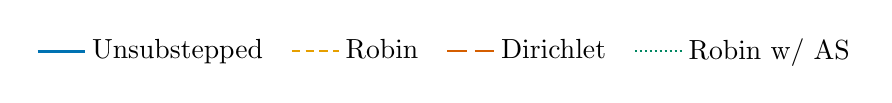
\begin{tikzpicture}[
    baseline,
    ]
  \begin{axis}[
    hide axis,
    xmin=0, xmax=1, ymin=0, ymax=1, % keeps the box tiny
    height=2cm,
    legend columns=-1,
    legend cell align=left,
    legend style={
      draw=none,
      /tikz/every even column/.append style={column sep=8pt},
    },
  ]

  % One dummy point per entry:
  \addplot[refstyle]      coordinates {(0,0)};
  \addlegendentry{Unsubstepped}

  \addplot[staggeredstyle] coordinates {(0,0)};
  \addlegendentry{Robin}

  \addplot[dirichletstyle] coordinates {(0,0)};
  \addlegendentry{Dirichlet}

  \addplot[chimerastyle]  coordinates {(0,0)};
  \addlegendentry{Robin w/ AS}

  \end{axis}
  \end{tikzpicture}\\
  \begin{subfigure}[t]{0.45\textwidth}
  \centering
  \begin{tikzpicture}[
      trim left={0mm},
      baseline,
      spy using outlines= {circle, connect spies}
      ]
    \begin{groupplot}[
      group style={
        group size=20 by 1,
        horizontal sep=0pt, % panels touch
        ylabels at=edge left,
        xlabels at=edge bottom
      },
      width=1.85cm,
      height=7cm,
    ]

    \addlayer{0}{pt1}{T}{\unit{\celsius}}{25}{1825}
    \addlayer{1}{pt1}{T}{\unit{\celsius}}{25}{1825}
    \addlayer{2}{pt1}{T}{\unit{\celsius}}{25}{1825}
    \addlayer{3}{pt1}{T}{\unit{\celsius}}{25}{1825}
    \addlayer{4}{pt1}{T}{\unit{\celsius}}{25}{1825}
    \addlayer{5}{pt1}{T}{\unit{\celsius}}{25}{1825}
    \addlayer{6}{pt1}{T}{\unit{\celsius}}{25}{1825}
    \addlayer{7}{pt1}{T}{\unit{\celsius}}{25}{1825}
    \addlayer{8}{pt1}{T}{\unit{\celsius}}{25}{1825}
    \addlayer{9}{pt1}{T}{\unit{\celsius}}{25}{1825}
    \addlayer{10}{pt1}{T}{\unit{\celsius}}{25}{1825}
    \addlayer{11}{pt1}{T}{\unit{\celsius}}{25}{1825}
    \addlayer{12}{pt1}{T}{\unit{\celsius}}{25}{1825}
    \addlayer{13}{pt1}{T}{\unit{\celsius}}{25}{1825}
    \addlayer{14}{pt1}{T}{\unit{\celsius}}{25}{1825}
    \addlayer{15}{pt1}{T}{\unit{\celsius}}{25}{1825}
    \addlayer{16}{pt1}{T}{\unit{\celsius}}{25}{1825}
    \addlayer{17}{pt1}{T}{\unit{\celsius}}{25}{1825}
    \addlayer{18}{pt1}{T}{\unit{\celsius}}{25}{1825}
    \addlayer{19}{pt1}{T}{\unit{\celsius}}{25}{1825}

    \end{groupplot}
    \node at ($(group c1r1.south)!0.5!(group c20r1.south)-(0,5mm)$) {\tiny Layer};
    \spy [black, width=2cm, height=2cm, magnification=3] on (spypoint) in node[fill=white] at (magnifyglass);

  \end{tikzpicture}
  \end{subfigure}%
  \hfill
  \begin{subfigure}[t]{0.45\textwidth}
  \centering
  \begin{tikzpicture}[
      trim left={0mm},
      baseline
      ]
    \begin{groupplot}[
      group style={
        group size=20 by 1,
        horizontal sep=0pt, % panels touch
        ylabels at=edge left,
        xlabels at=edge bottom
      },
      width=1.85cm,
      height=7cm,
    ]

    \addlayer{0}{W}{Melt pool width}{\unit{\milli\meter}}{0.0}{0.35}
    \addlayer{1}{W}{Melt pool width}{\unit{\milli\meter}}{0.0}{0.35}
    \addlayer{2}{W}{Melt pool width}{\unit{\milli\meter}}{0.0}{0.35}
    \addlayer{3}{W}{Melt pool width}{\unit{\milli\meter}}{0.0}{0.35}
    \addlayer{4}{W}{Melt pool width}{\unit{\milli\meter}}{0.0}{0.35}
    \addlayer{5}{W}{Melt pool width}{\unit{\milli\meter}}{0.0}{0.35}
    \addlayer{6}{W}{Melt pool width}{\unit{\milli\meter}}{0.0}{0.35}
    \addlayer{7}{W}{Melt pool width}{\unit{\milli\meter}}{0.0}{0.35}
    \addlayer{8}{W}{Melt pool width}{\unit{\milli\meter}}{0.0}{0.35}
    \addlayer{9}{W}{Melt pool width}{\unit{\milli\meter}}{0.0}{0.35}
    \addlayer{10}{W}{Melt pool width}{\unit{\milli\meter}}{0.0}{0.35}
    \addlayer{11}{W}{Melt pool width}{\unit{\milli\meter}}{0.0}{0.35}
    \addlayer{12}{W}{Melt pool width}{\unit{\milli\meter}}{0.0}{0.35}
    \addlayer{13}{W}{Melt pool width}{\unit{\milli\meter}}{0.0}{0.35}
    \addlayer{14}{W}{Melt pool width}{\unit{\milli\meter}}{0.0}{0.35}
    \addlayer{15}{W}{Melt pool width}{\unit{\milli\meter}}{0.0}{0.35}
    \addlayer{16}{W}{Melt pool width}{\unit{\milli\meter}}{0.0}{0.35}
    \addlayer{17}{W}{Melt pool width}{\unit{\milli\meter}}{0.0}{0.35}
    \addlayer{18}{W}{Melt pool width}{\unit{\milli\meter}}{0.0}{0.35}
    \addlayer{19}{W}{Melt pool width}{\unit{\milli\meter}}{0.0}{0.35}

    \end{groupplot}
    \node at ($(group c1r1.south)!0.5!(group c20r1.south)-(0,5mm)$) {\tiny Layer};

  \end{tikzpicture}
  \end{subfigure}
  \caption{Temperature history at a point (left)
    and melt pool width (right)
    throughout the print of the 1.0 \unit{\milli\meter}
    cube using $\Delta t_s = 10 T_{hs}$.
    The probe is located at the center of the top surface of the substrate,
    that is, right below the first layer.
    Cooling intervals are excluded for clarity.
  }
  \label{fig:3d_lpbf_probe}
\end{figure}

\end{frame}

\begin{frame}
  \frametitle{Substepping}
  \framesubtitle{3D LPBF cube}
  \begin{itemize}
    \item Speed-up factors range from about $1.3$--$2.0$ for fast DOF ratios around
    $30\%$, up to roughly $4$--$6.5$ when the fast DOF ratio drops below
    $10\%$, depending on substepper and use of AS.
    \item Robin substepping slightly outperforms Dirichlet.
    \item AS approach yields increasing speed-ups with domain size; substantial gains for cubes $\geq 2\,\si{\milli\meter}$.
    \item For short tracks and large macro-steps, fast-domain DOF fraction can exceed profitability threshold and reduce speed-up.
    \item AS distorts thermal tail when advected subdomain overlaps previous tracks.
  \end{itemize}
\end{frame}

\begin{frame}
  \frametitle{Substepping + advected subdomain}
  \framesubtitle{Final conclusions}
  \begin{itemize}
    \item The AS method improved HAZ accuracy and allowed much larger
      time-steps (up to several \(T_{hs}\)), at the cost of losing SPD
      structure and increasing per-step cost by roughly a factor of 2–3.
    \item AS works best on long, simple tracks; direction
      changes and overlapping tracks shear thermal tails and can severely
      degrade accuracy, limiting applicability as a general speed-up
      technique.
    \item Substepping, via fast/slow domain partitioning with
      \(\Delta t_f\) and \(\Delta t_s \gg \Delta t_f\), provided a more
      robust and broadly applicable way to exploit time-scale disparity in
      LPBF.
    \end{itemize}
  \end{frame}
